% !TeX program = xelatex
% =============================================================================
%  DỰ ÁN TỐT NGHIỆP — BÁO CÁO CHUYÊN ĐỀ
%  Đề tài: Phân tích Hiệu suất và Dự báo Sản lượng Hệ thống Điện Mặt Trời
%  Nhóm: The Outliers
%  Trường: Cao đẳng FPT Polytechnic — Chuyên ngành Xử lý Dữ liệu
% =============================================================================

\documentclass[12pt, a4paper]{report}

% ======================== PACKAGES CƠ BẢN & FONT ============================
\usepackage{geometry}
\geometry{a4paper, top=2.5cm, bottom=2.5cm, left=3cm, right=2cm, headheight=33pt, footskip=1.1cm}

% --- FONT CHO XELATEX (HỖ TRỢ TIẾNG VIỆT 100% - FORMAL, TỐI GIẢN, HIỆN ĐẠI) ---
\usepackage{fontspec}
\setmainfont{Times New Roman}
\setmonofont{Consolas}

% ======================== MÀU SẮC & CODE LISTINGS ===========================
\usepackage{xcolor}
\usepackage{listings}
% Định nghĩa bảng màu Tableau trích xuất từ main_fixed_01.twb & tableau_theme.json
\definecolor{tblNavy}{HTML}{4E79A7}
\definecolor{tblOrange}{HTML}{F28E2B}
\definecolor{tblGreen}{HTML}{59A14F}
\definecolor{tblRed}{HTML}{E15759}
\definecolor{tblTeal}{HTML}{76B7B2}
\definecolor{tblYellow}{HTML}{EDC948}
\definecolor{tblPurple}{HTML}{B07AA1}
\definecolor{tblGray}{HTML}{79706E}
\definecolor{tblSeqWarm}{HTML}{F28E2B}

% Định nghĩa màu sắc cho Code Block
\definecolor{mutedgreen}{rgb}{0.2,0.5,0.3} 
\definecolor{mutedblue}{rgb}{0.15,0.35,0.6} 
\definecolor{mutedgray}{rgb}{0.45,0.45,0.45} 
\definecolor{mutedpurple}{rgb}{0.45,0.2,0.55} 
\definecolor{softbackground}{rgb}{0.98,0.98,0.98} 
\definecolor{bordergray}{rgb}{0.85,0.85,0.85} 
\definecolor{fptorange}{RGB}{245,130,32}

\lstdefinestyle{pythonstyle}{
    backgroundcolor   = \color{softbackground},
    commentstyle      = \color{mutedgreen}\itshape,
    keywordstyle      = \color{mutedblue}\bfseries,
    numberstyle       = \tiny\color{mutedgray},
    stringstyle       = \color{mutedpurple},
    basicstyle        = \ttfamily\footnotesize\color{black},
    breakatwhitespace = false,
    breaklines        = true,
    columns           = fullflexible,
    captionpos        = t, 
    keepspaces        = true,
    numbers           = left,
    numbersep         = 5pt,
    showspaces        = false,
    showstringspaces  = false,
    showtabs          = false,
    tabsize           = 4,
    frame             = single,
    rulecolor         = \color{bordergray}
}
\lstset{style=pythonstyle}

% Ngăn chặn tự động gạch nối từ (hyphenation) cuối dòng
\hyphenpenalty=10000
\exhyphenpenalty=10000
\tolerance=10000
\emergencystretch=3em

% ======================== TRANG TRÍ & ĐỊNH DẠNG =============================
\usepackage{fancyhdr}
\usepackage{lastpage}
\usepackage{amsmath, amssymb}
\usepackage{enumitem}
\usepackage{array}
\newcolumntype{L}[1]{>{\raggedright\arraybackslash}p{#1}}
\newcolumntype{C}[1]{>{\centering\arraybackslash}p{#1}}
\newcolumntype{R}[1]{>{\raggedleft\arraybackslash}p{#1}}
\usepackage{booktabs}
\usepackage{tabularx}
\usepackage{longtable}
\usepackage{multirow}
\usepackage{graphicx}
\graphicspath{{images/}{figures/}{./}}
\usepackage{float}
\usepackage{caption}
\usepackage{subcaption}
\usepackage{tikz}
\usepackage[titles]{tocloft}

% VIỆT HÓA TOÀN BỘ CÁC TIÊU ĐỀ HỆ THỐNG
\renewcommand{\figurename}{Hình}
\renewcommand{\tablename}{Bảng}
\renewcommand{\contentsname}{Mục Lục}
\renewcommand{\listfigurename}{Danh Mục Hình Vẽ}
\renewcommand{\listtablename}{Danh Mục Bảng Biểu}
\providecommand{\tep}[1]{\texttt{#1}}

\usepackage{indentfirst}
\setlength{\parindent}{1cm}
\setlength{\parskip}{6pt}

\usepackage{setspace}
\onehalfspacing
\setlength{\headheight}{33pt}

% Hyperlinks & Bookmarks
\usepackage{hyperref}
\hypersetup{
    colorlinks  = true,
    linkcolor   = black,
    citecolor   = blue,
    filecolor   = magenta,
    urlcolor    = blue,
    pdftitle    = {Dự án Tốt nghiệp - Phân tích Hiệu suất và Dự báo Sản lượng Hệ thống Điện Mặt Trời},
    pdfauthor   = {The Outliers - FPT Polytechnic},
    bookmarksnumbered = true,
}

% --- CẤU HÌNH TIÊU ĐỀ CHƯƠNG ---
\usepackage{placeins}
\makeatletter
\newcommand{\needspace}[1]{%
  \begingroup
    \setlength{\dimen@}{#1}%
    \vskip\z@\@plus\dimen@
    \penalty -100\vskip\z@\@plus -\dimen@
    \vskip\dimen@
    \penalty 9999\vskip -\dimen@
    \vskip\z@skip
  \endgroup}
\makeatother
\usepackage{titlesec}
\titleformat*{\section}{\fontsize{13pt}{15.6pt}\bfseries}
\titleformat*{\subsection}{\fontsize{13pt}{15.6pt}\bfseries}
\titleformat*{\subsubsection}{\fontsize{13pt}{15.6pt}\bfseries}
\titleformat{\chapter}[display]
  {\normalfont\huge\bfseries}{}{0pt}{\huge}
\titlespacing*{\chapter}{0pt}{-10pt}{20pt} 

% ======================== HEADER / FOOTER ====================================
\fancypagestyle{main}{
    \fancyhf{}
    \fancyhead[L]{
\includegraphics[height=1cm]{figures/logo_fpoly.png}}
    \fancyhead[R]{\small THE OUTLIERS}
    \fancyfoot[L]{\small Dự án Tốt nghiệp — Chuyên ngành Xử lý Dữ liệu}
    \fancyfoot[R]{\small Trang \thepage\ / \pageref{LastPage}}
    \renewcommand{\headrulewidth}{0.4pt}
    \renewcommand{\footrulewidth}{0.4pt}
}

\fancypagestyle{plain}{
    \fancyhf{}
    \fancyfoot[L]{\small Dự án Tốt nghiệp — Chuyên ngành Xử lý Dữ liệu}
    \fancyfoot[R]{\small Trang \thepage\ / \pageref{LastPage}}
    \renewcommand{\headrulewidth}{0pt}
    \renewcommand{\footrulewidth}{0.4pt}
}

\fancypagestyle{front}{
    \fancyhf{}
    \fancyfoot[L]{\small Dự án Tốt nghiệp — Chuyên ngành Xử lý Dữ liệu}
    \fancyfoot[R]{\small Trang \thepage\ / \pageref{LastPage}}
    \renewcommand{\headrulewidth}{0pt}
    \renewcommand{\footrulewidth}{0.4pt}
}


\begin{document}
\pagestyle{front}

\begin{titlepage}
\enlargethispage{1.2cm}

\begin{tikzpicture}[remember picture, overlay]
    \draw[line width=2pt, fptorange]
        ([shift={(1cm,-1cm)}]current page.north west)
        rectangle
        ([shift={(-1cm,1cm)}]current page.south east);
    \draw[line width=0.5pt, fptorange]
        ([shift={(1.15cm,-1.15cm)}]current page.north west)
        rectangle
        ([shift={(-1.15cm,1.15cm)}]current page.south east);
\end{tikzpicture}

\begin{center}
    \textbf{\large TRƯỜNG CAO ĐẲNG FPT POLYTECHNIC}

    \vspace{0.5cm}
    
\includegraphics[width=0.38\textwidth]{figures/logo_fpoly.png}

    \vspace{0.4cm}
    {\Large \textbf{DỰ ÁN TỐT NGHIỆP}} \\[4pt]
    {\large \textbf{CHUYÊN NGÀNH: XỬ LÝ DỮ LIỆU}}

    \vspace{1.6cm}
    
    \begin{spacing}{1.0}
        {\huge \textbf{PHÂN TÍCH HIỆU SUẤT VÀ \\[4pt] DỰ BÁO SẢN LƯỢNG \\[4pt] HỆ THỐNG ĐIỆN MẶT TRỜI}}
    \end{spacing}

    \vspace{1.8cm}
    \normalsize
    \begin{flushleft}
        \hspace{2cm} \textbf{Nhóm thực hiện:} The Outliers \\[5pt]
        \hspace{2cm} \textbf{Sinh viên thực hiện:} \\[3pt]
        \hspace{2cm}
        \begin{tabular*}{7.5cm}{@{} l @{\extracolsep{\fill}} r @{}}
            \hspace{0.5cm} 1. Nguyễn Vũ Nhựt   & PS44442 \\
            \hspace{0.5cm} 2. Nguyễn Văn Sỹ    & PS43671 \\
            \hspace{0.5cm} 3. Lê Công Toàn    & PS44145 \\
            \hspace{0.5cm} 4. Nguyễn Xuân Hùng & PS44527 \\
            \hspace{0.5cm} 5. Ngô Tấn Đạt     & PS44589 \\
        \end{tabular*} \\[5pt]
        \hspace{2cm} \textbf{Giảng viên hướng dẫn:} Văn Công Khanh
    \end{flushleft}
    \vfill
    {\normalsize \textbf{TP. HỒ CHÍ MINH, THÁNG 6 NĂM 2026}}
    \vspace{0.5cm}
\end{center}
\end{titlepage}


\pagenumbering{arabic}
\pagestyle{main}

\chapter{Khai phá Dữ liệu và Mô hình Dự báo Sản lượng}
\label{chap:forecasting}

\section{Tổng quan Bài toán và Quy trình Học máy (MLOps Pipeline)}
\label{sec:ml_overview}

\subsection{Phát biểu Bài toán và Phạm vi Dự báo}
Dự báo sản lượng điện mặt trời là bài toán hồi quy chuỗi thời gian đa biến có tính bất định cao do phụ thuộc chặt chẽ vào các yếu tố khí tượng và trạng thái thiết bị. Dự án tập trung giải quyết bài toán dự báo đa bước thời gian (Multi-horizon Time-Series Forecasting) tại 2 tầm nhìn tác chiến:
\begin{itemize}[noitemsep]
    \item \textbf{Tầm nhìn Ngắn hạn ($H = 1$, tức $15$ phút tiếp theo):} Phục vụ điều độ hòa lưới thời gian thực, cân bằng công suất biến tần và cảnh báo suy giảm đột ngột.
    \item \textbf{Tầm nhìn Trung hạn ($H = 4$, tức $1$ giờ tiếp theo):} Hỗ trợ kế hoạch huy động nguồn điện dự phòng, tối ưu hóa phụ tải khuôn viên và tham gia thị trường điện.
\end{itemize}

Đầu vào của mô hình là tập dữ liệu hợp nhất \path{data/mlmart_base/v4_final_cleaned.parquet} gồm $2.731.946$ bản ghi độ phân giải $15$ phút, thu thập từ $42$ trạm phát điện mặt trời tại 5 khuôn viên thuộc Đại học La Trobe, Úc (công bố bởi Wimalaratne và cộng sự~\cite{wimalaratne2022unisolar}, Hình~\ref{fig:unisolar}), kết hợp với chuỗi $15$ tham số khí tượng lịch sử từ Open-Meteo API~\cite{openmeteo2023}.

\begin{figure}[H]
    \centering
    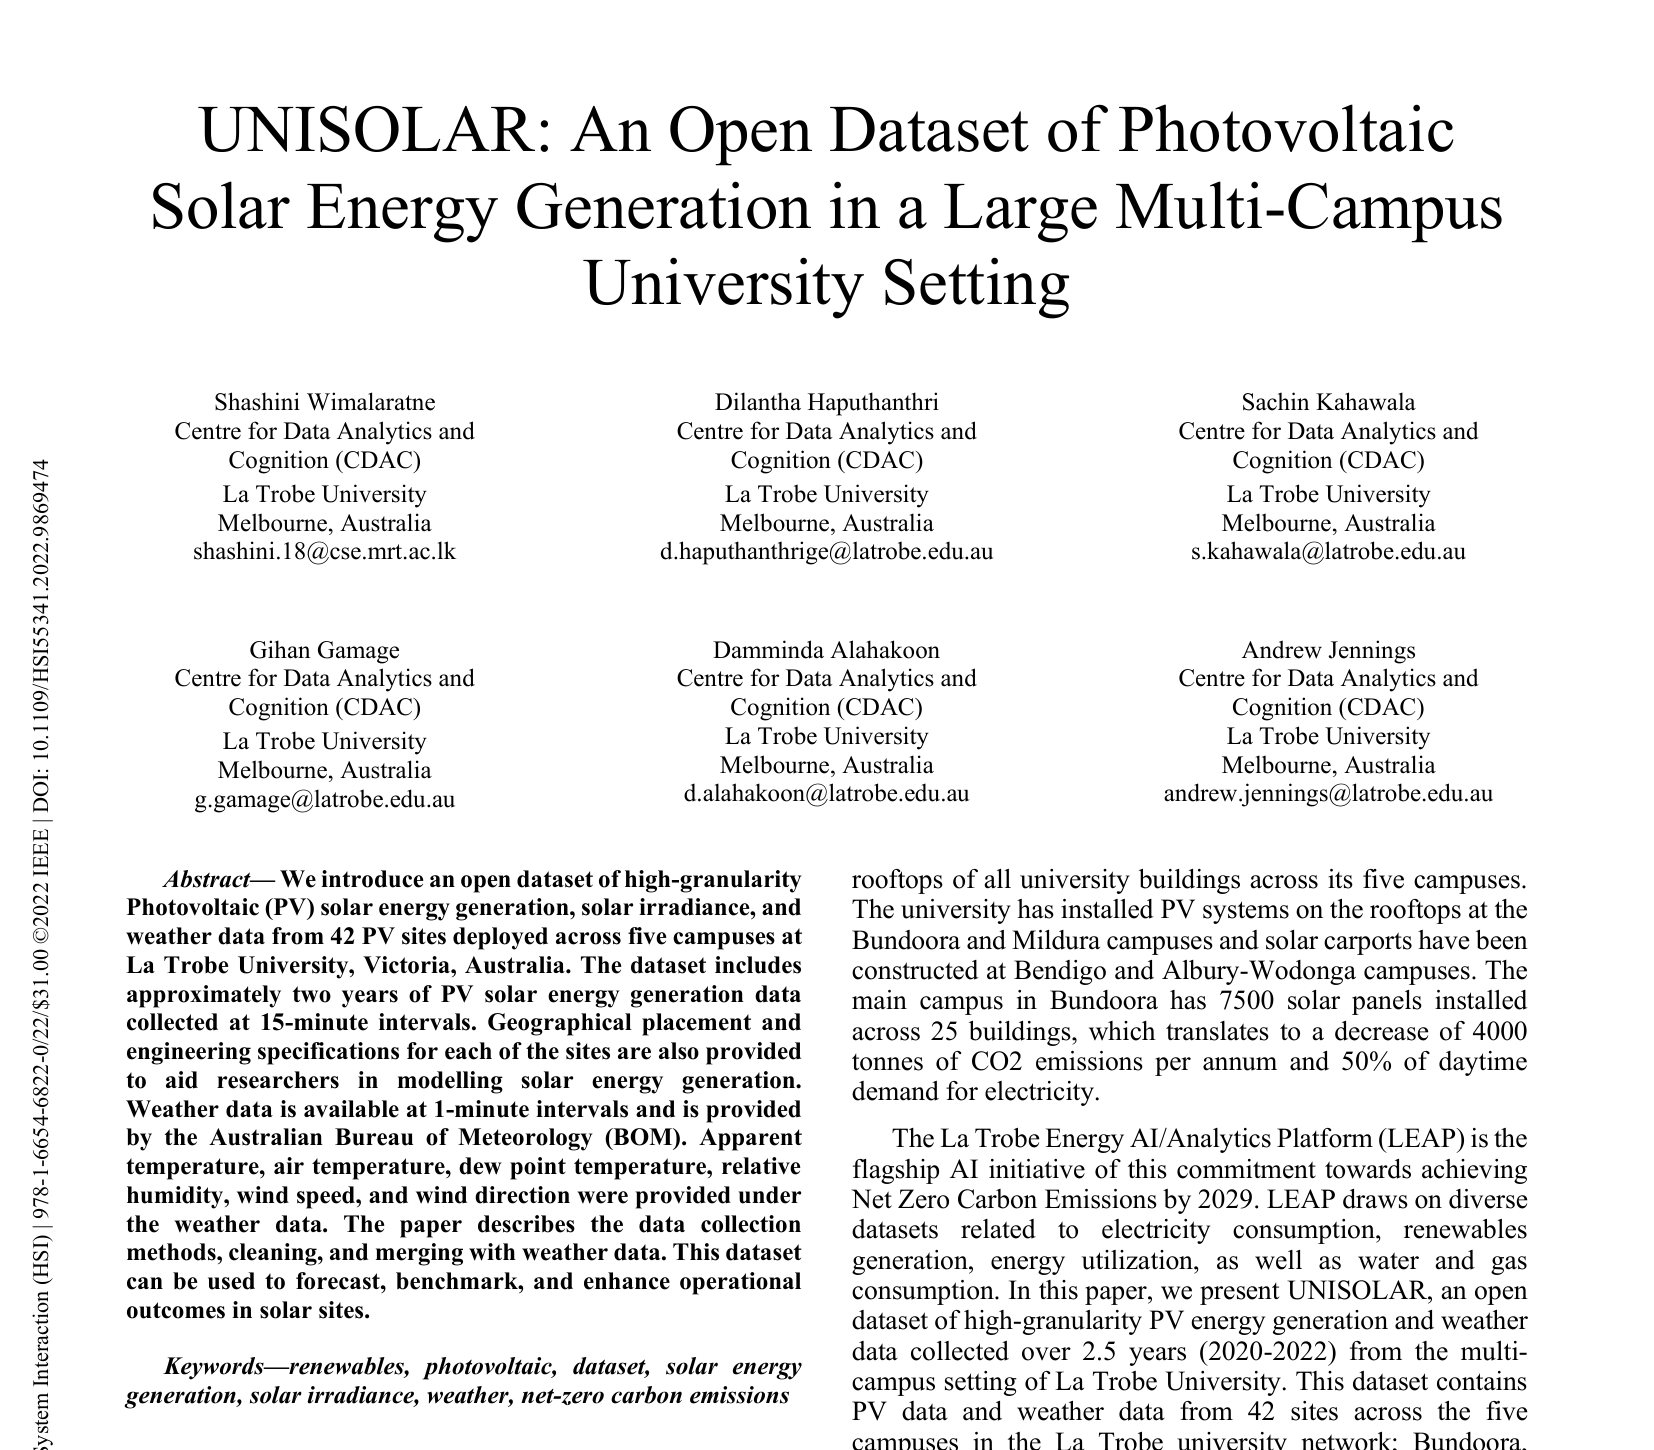
\includegraphics[width=0.88\textwidth]{paper_unisolar_dataset.png}
    \caption{Tài liệu công bố tập dữ liệu mở UNISOLAR ($42$ trạm phát, $5$ khuôn viên, chu kỳ $15$ phút)~\cite{wimalaratne2022unisolar}.}
    \label{fig:unisolar}
\end{figure}

\subsection{Kiến trúc Quy trình MLOps và Rào chắn Chống Rò rỉ Thông tin}
Để đảm bảo tính tái lập và độ tin cậy trong môi trường sản xuất thực tế, toàn bộ quy trình từ tiền xử lý, kỹ sư đặc trưng, huấn luyện mô hình đến giải thích kết quả được đóng gói tự động hóa thành Pipeline theo chuẩn MLOps (Hình~\ref{fig:mlops_pipeline}).

\begin{figure}[H]
    \centering
    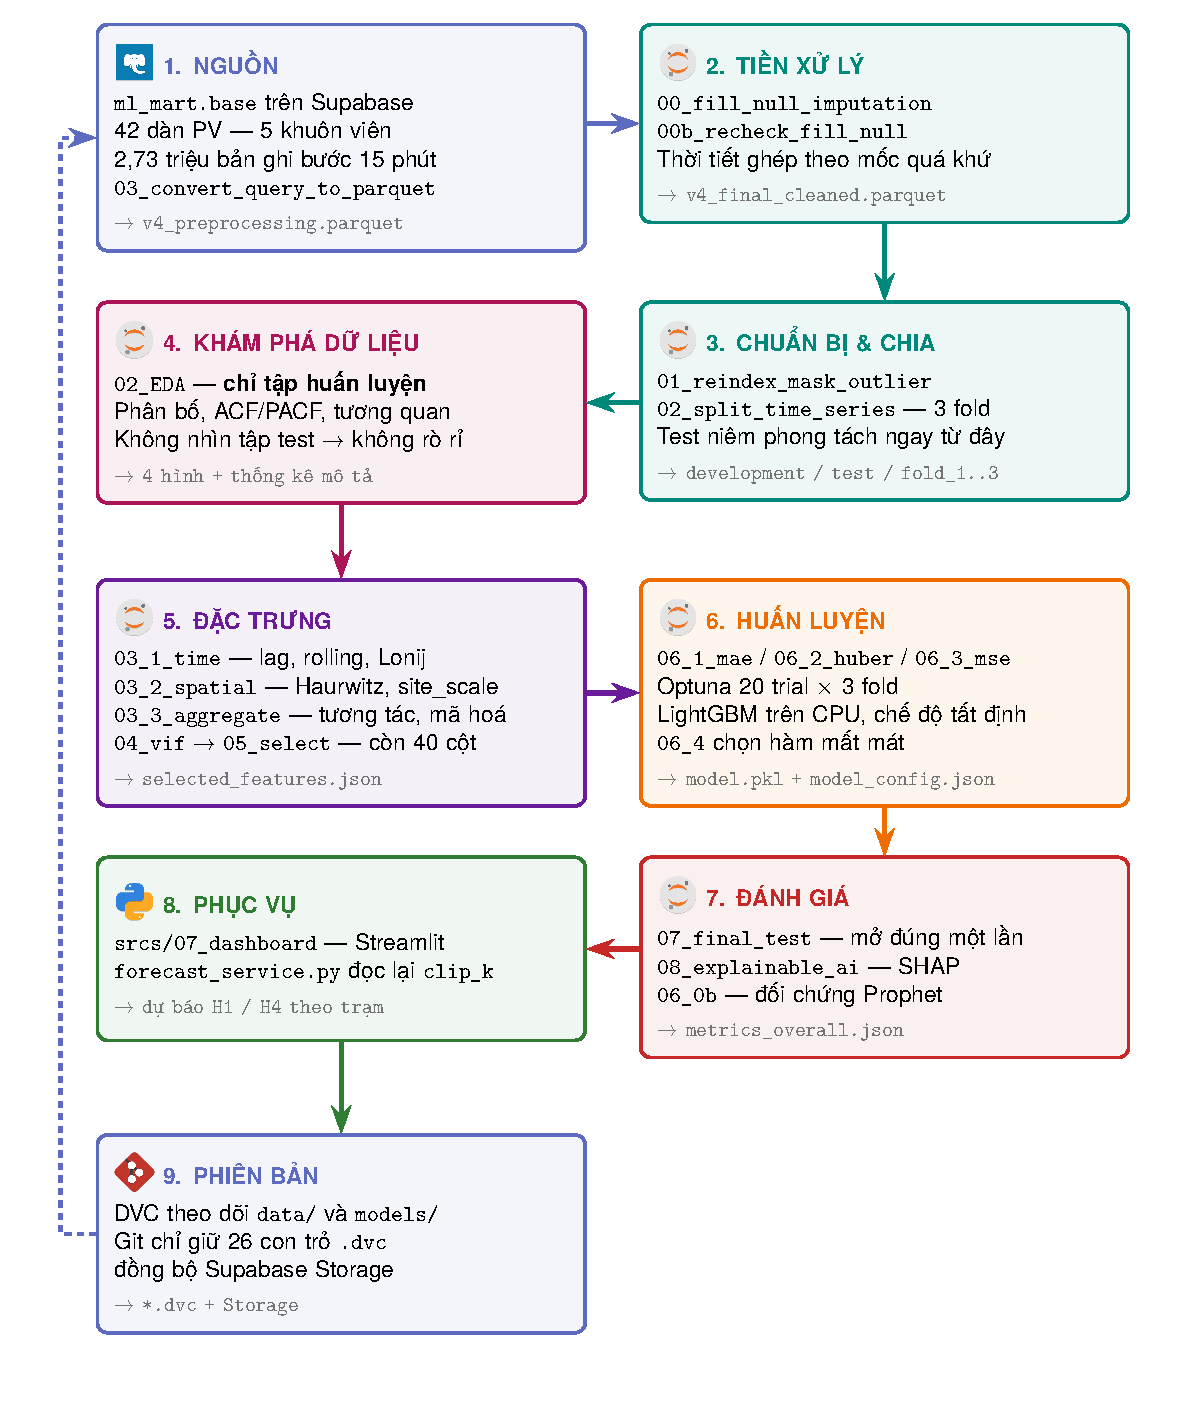
\includegraphics[width=0.92\textwidth]{pipeline_sodo_mlops.pdf}
    \caption{Sơ đồ kiến trúc quy trình học máy tự động hóa (MLOps Pipeline).}
    \label{fig:mlops_pipeline}
\end{figure}

Năm rào chắn vật lý và logic chống rò rỉ dữ liệu (Data Leakage Guards) được áp dụng nghiêm ngặt:
\begin{enumerate}[label=\arabic*., leftmargin=*]
    \item \textbf{Rào chắn Thời gian (Strict Temporal Ordering):} Tại thời điểm dự báo $T$, mô hình chỉ được phép tiếp cận dữ liệu quá khứ ($t \le T$). Mọi phép tính thống kê trượt và trễ thời gian đều dịch lùi tối thiểu 1 bước đo.
    \item \textbf{Khí tượng Causal-only:} Tuyệt đối không sử dụng giá trị khí tượng tương lai chưa được kiểm chứng; chỉ sử dụng dự báo thời tiết tại thời điểm $T$ hoặc quan trắc quá khứ.
    \item \textbf{Đóng băng Hệ số Chuẩn hóa (Frozen Scale Factor):} Các tham số thống kê quy mô trạm (\texttt{site\_scale}, công suất danh định $P_{\text{stc}}$) chỉ được tính toán trên tập Huấn luyện (Train set) và đóng băng khi áp dụng vào tập Kiểm thử (Test set).
    \item \textbf{Khóa Kín Tập Test (Sealed Test Set):} Tập Test được cô lập hoàn toàn, không tham gia vào bất kỳ khâu chuẩn hóa dữ liệu, chọn đặc trưng hay tối ưu siêu tham số nào.
    \item \textbf{Cách ly Outlier trong Đánh giá:} Dữ liệu ngoại lai do hỏng hóc cảm biến hoặc dừng máy bảo trì được gắn cờ \texttt{gmm\_if\_outlier\_flag} để loại trừ khỏi khâu huấn luyện, nhưng vẫn được giữ lại để đánh giá năng lực nhận diện lỗi của hệ thống.
\end{enumerate}

\section{Phân chia Dữ liệu và Điền khuyết Nhân quả (Causal Imputation)}
\label{sec:data_prep_imputation}

\subsection{Chiến lược Phân chia Chuỗi Thời gian (Temporal Split)}
Nhằm phản ánh đúng điều kiện vận hành trong thực tế, dự án sử dụng phương pháp phân chia chuỗi thời gian thuần túy theo dòng thời gian (Purged Temporal Train-Test Split):
\begin{itemize}[noitemsep]
    \item \textbf{Tập Phát triển (Development Set -- $80\%$):} Từ ngày $01/01/2020$ đến $30/06/2022$, gồm $2.273.970$ bản ghi. Tập này được dùng để huấn luyện mô hình, kiểm tra chéo (3-Fold Expanding Window Cross-Validation) và tinh chỉnh siêu tham số.
    \item \textbf{Tập Kiểm thử Độc lập (Sealed Test Set -- $20\%$):} Từ ngày $01/07/2022$ đến $31/12/2022$, gồm $510.468$ bản ghi. Tập này được giữ kín tuyệt đối để chấm điểm khách quan.
\end{itemize}

\subsection{Bậc thang Điền khuyết Nhân quả (Causal Cascade Imputation)}
Dữ liệu thô tồn tại $52.492$ khoảng trống thời gian (Time Gaps) cần được lấp đầy để duy trì tính liên tục cho các phép tính trễ và cửa sổ trượt. Theo khuyến nghị của Kim et al. (2019)~\cite{kim2019missing}, dự án xây dựng thuật toán điền khuyết theo bậc thang nhân quả (Causal Cascade), tuyệt đối không dùng nội suy nhìn về tương lai (Linear Interpolation):
\begin{enumerate}[label=\arabic*., leftmargin=*]
    \item \textbf{Mức 1 -- Ban đêm (\texttt{night\_zero}):} Nếu bức xạ $GHI = 0\,\text{W/m}^2$ và góc cao mặt trời $h \le 0^\circ$, gán $E = 0\,\text{kWh}$.
    \item \textbf{Mức 2 -- Quá khứ Ngày hôm trước (\texttt{causal\_day\_persistence}):} Lấy giá trị tại cùng thời điểm ngày hôm trước ($T - 24\,\text{h}$).
    \item \textbf{Mức 3 -- Quá khứ Tuần trước (\texttt{causal\_week\_persistence}):} Lấy giá trị tại cùng thời điểm tuần trước ($T - 168\,\text{h}$).
    \item \textbf{Mức 4 -- Trung vị Lịch sử (\texttt{causal\_profile\_median}):} Lấy trung vị của cùng khung giờ trong tháng thuộc tập Train.
    \item \textbf{Mức 5 -- Dự phòng (\texttt{fallback\_zero}):} Gán giá trị $0$ cho các điểm bất khả kháng còn sót lại.
    \item \textbf{Mức 6 -- Sự cố Dừng máy (\texttt{machine\_failure\_zero}):} Các khoảng mất dữ liệu kéo dài trên $24\,\text{h}$ liên tục được định danh là sự cố bảo trì thiết bị và đánh dấu loại bỏ khỏi tập học.
\end{enumerate}

\section{Kỹ thuật Đặc trưng và Chẩn đoán Đa cộng tuyến (Feature Engineering \& VIF)}
\label{sec:feature_engineering}

\subsection{Không gian Đặc trưng Đa chiều}
Dự án trích xuất $75$ đặc trưng khởi tạo, kết hợp giữa tri thức vật lý quang điện và các biến đổi chuỗi thời gian:
\begin{itemize}[noitemsep]
    \item \textbf{Nhóm Thời gian \& Chu kỳ (Temporal Cycles):} \texttt{minute\_of\_day}, \texttt{hour\_sin}, \texttt{hour\_cos}, \texttt{doy\_sin}, \texttt{doy\_cos}, \texttt{is\_weekend}. Mã hóa dạng sin/cos giúp mô hình hiểu tính tuần hoàn liên tục của ngày và năm.
    \item \textbf{Nhóm Mô hình Bầu trời Quang (Clear-Sky Model Haurwitz 1945~\cite{haurwitz1945}):} Tính toán bức xạ lý thuyết không mây $GHI_{\text{cs}} = 1098 \cdot \sin(h) \cdot \exp(-0{,}059/\sin(h))$, góc cao mặt trời $\sin(h)$, và chỉ số trời quang $k_{\text{target}} = E / (P_{\text{stc}} \cdot \max(\sin h, \varepsilon))$.
    \item \textbf{Nhóm Quy mô Trạm (Spatial Normalization):} Chuẩn hóa sản lượng theo công suất lắp đặt trạm \texttt{site\_scale} và hệ số bão hòa biến tần \texttt{ty\_le\_bao\_hoa}.
    \item \textbf{Nhóm Trễ Nhân quả \& Thống kê Trượt (Causal Lags \& Rolling Statistics):} \texttt{lag\_4} ($T - 60\,\text{phút}$), \texttt{lag\_96} ($T - 24\,\text{giờ}$), cùng các thống kê trượt \texttt{rolling\_mean\_4}, \texttt{rolling\_std\_4}, \texttt{rolling\_min\_4}, \texttt{rolling\_max\_4} trên cửa sổ 1 giờ.
    \item \textbf{Nhóm Tương tác Khí tượng (Physical Interactions):} Tích giữa bức xạ và nhiệt độ ($GHI \times \text{temp}$), tỷ lệ bức xạ tán xạ ($DHI / GHI$), và độ che phủ mây ($cloud \times GHI$).
\end{itemize}

\subsection{Chẩn đoán Đa cộng tuyến (VIF) và Lựa chọn Đặc trưng Tối ưu}
Các biến thời tiết và bức xạ thường có mối tương quan tuyến tính rất mạnh. Nhóm thực hiện chẩn đoán hệ số phóng đại phương sai (Variance Inflation Factor -- VIF) và chắt lọc danh sách xuống còn 40 đặc trưng tối ưu (Bảng~\ref{tab:selected_40_features}) với $VIF < 10$, triệt tiêu hoàn toàn hiện tượng đa cộng tuyến và tối ưu hóa thời gian huấn luyện.

\begin{table}[H]
\centering
\small
\renewcommand{\arraystretch}{1.2}
\begin{tabularx}{\textwidth}{@{} l p{4.2cm} X @{}}
\toprule
\textbf{Nhóm Đặc trưng} & \textbf{Số lượng Cột} & \textbf{Các Biến Tiêu biểu trong Mô hình} \\
\midrule
Thời gian \& Chu kỳ & 10 đặc trưng & \texttt{minute\_of\_day}, \texttt{hour\_sin}, \texttt{hour\_cos}, \texttt{doy\_sin}, \texttt{doy\_cos}, \texttt{is\_weekend}, \texttt{month} \\
\midrule
Vật lý Bầu trời quang & 8 đặc trưng & \texttt{ghi\_cs}, \texttt{sin\_elevation}, \texttt{solar\_azimuth}, \texttt{azimuth\_sin}, \texttt{azimuth\_cos}, \texttt{clearsky\_proxy} \\
\midrule
Khí tượng Viễn thám & 6 đặc trưng & \texttt{shortwave\_radiation} ($GHI$), \texttt{direct\_normal\_irradiance} ($DNI$), \texttt{diffuse\_solar\_radiation} ($DHI$), \texttt{temperature\_c}, \texttt{cloud\_cover\_total} \\
\midrule
Trễ \& Cửa sổ trượt & 6 đặc trưng & \texttt{lag\_4}, \texttt{lag\_96}, \texttt{rolling\_mean\_4}, \texttt{rolling\_std\_4}, \texttt{rolling\_min\_4}, \texttt{rolling\_max\_4} \\
\midrule
Tương tác Vật lý & 6 đặc trưng & \texttt{temp\_x\_shortwave}, \texttt{diffuse\_ratio}, \texttt{cloud\_x\_shortwave}, \texttt{rad\_x\_sinelev}, \texttt{ty\_le\_bao\_hoa} \\
\midrule
Quy mô Trạm \& Vận hành & 4 đặc trưng & \texttt{site\_scale}, \texttt{tran\_cong\_suat}, \texttt{capacity\_kw}, \texttt{number\_of\_panels} \\
\bottomrule
\end{tabularx}
\caption{Tổng hợp không gian $40$ đặc trưng tối ưu được chọn sau bước chẩn đoán VIF.}
\label{tab:selected_40_features}
\end{table}

\section{Huấn luyện Mô hình, Tối ưu Siêu tham số và So sánh Đối chứng}
\label{sec:model_training_tuning}

\subsection{Kiến trúc Mô hình Cốt lõi: LightGBM Regressor}
Dự án lựa chọn thuật toán LightGBM (Light Gradient Boosting Machine)~\cite{ke2017lightgbm} làm mô hình dự báo chủ đạo nhờ các ưu điểm vượt trội:
\begin{itemize}[noitemsep]
    \item Kỹ thuật phát triển cây theo chiều sâu tối ưu lá (Leaf-wise Tree Growth) giúp cực tiểu hóa hàm mất mát nhanh hơn cơ chế Depth-wise truyền thống.
    \item Hỗ trợ hàm mất mát mạnh mẽ (Robust Loss): Sử dụng Huber Loss ($\alpha = 0{,}95$) và L1 Loss (MAE) giúp mô hình miễn nhiễm với các điểm ngoại lai đo đạc đột biến.
    \item Tốc độ tính toán và hiệu quả bộ nhớ xuất sắc, cho phép xử lý mượt mà toàn bộ $2{,}73$ triệu dòng dữ liệu trên phần cứng tiêu chuẩn.
\end{itemize}

\subsection{Tối ưu hóa Siêu tham số Tự động bằng Optuna}
Nhóm sử dụng khung tối ưu Bayesian Optimization (Optuna) qua $50$ lượt thử nghiệm (Trials) với chiến lược kiểm tra chéo 3-Fold Expanding Window. Bảng~\ref{tab:optuna_hyperparameters} liệt kê không gian tìm kiếm và bộ siêu tham số tối ưu đạt được:

\begin{table}[H]
\centering
\small
\renewcommand{\arraystretch}{1.25}
\begin{tabularx}{\textwidth}{@{} l l l X @{}}
\toprule
\textbf{Siêu tham số} & \textbf{Miền Tìm kiếm} & \textbf{Giá trị Tối ưu} & \textbf{Ý nghĩa Kỹ thuật} \\
\midrule
\texttt{learning\_rate} & $[0{,}01,\, 0{,}10]$ & $\mathbf{0{,}03}$ & Tốc độ học kiểm soát độ co giãn trọng số của từng cây boosting. \\
\texttt{num\_leaves} & $[31,\, 127]$ & $\mathbf{63}$ & Số lượng lá tối đa trong một cây, kiểm soát độ phức tạp mô hình. \\
\texttt{max\_depth} & $[6,\, 12]$ & $\mathbf{8}$ & Độ sâu tối đa để ngăn ngừa hiện tượng học vẹt (Overfitting). \\
\texttt{subsample} & $[0{,}6,\, 1{,}0]$ & $\mathbf{0{,}80}$ & Tỷ lệ lấy mẫu ngẫu nhiên dữ liệu huấn luyện cho mỗi vòng lặp. \\
\texttt{colsample\_bytree} & $[0{,}6,\, 1{,}0]$ & $\mathbf{0{,}80}$ & Tỷ lệ lấy mẫu đặc trưng tại mỗi nhánh phân tách. \\
\texttt{reg\_alpha} (L1) & $[10^{-3},\, 10^{1}]$ & $\mathbf{0{,}10}$ & Trọng số suy giảm L1 hỗ trợ làm thưa đặc trưng (Feature Sparsity). \\
\texttt{reg\_lambda} (L2) & $[10^{-3},\, 10^{1}]$ & $\mathbf{1{,}00}$ & Trọng số phạt L2 chống bùng nổ trọng số lá. \\
\bottomrule
\end{tabularx}
\caption{Không gian tìm kiếm và cấu hình siêu tham số tối ưu tìm được qua Optuna.}
\label{tab:optuna_hyperparameters}
\end{table}

\subsection{Hệ thống Mô hình Đối chứng (Baselines)}
Để đánh giá chính xác năng lực gia tăng giá trị của mô hình học máy, nhóm thiết lập 4 mô hình đối chứng chuẩn:
\begin{enumerate}[label=\arabic*., leftmargin=*]
    \item \textbf{Naive Persistence Baseline:} Dự báo giá trị tại $T + h$ bằng đúng giá trị quan trắc tại thời điểm hiện tại $T$: $\hat{y}_{T+h} = y_T$.
    \item \textbf{Daily Persistence Baseline:} Dự báo bằng giá trị cùng thời điểm này ngày hôm trước: $\hat{y}_{T+h} = y_{T+h - 24\text{h}}$.
    \item \textbf{Weekly Persistence Baseline:} Dự báo bằng giá trị cùng thời điểm tuần trước: $\hat{y}_{T+h} = y_{T+h - 168\text{h}}$.
    \item \textbf{Facebook Prophet with Exogenous Weather~\cite{taylor2018prophet}:} Mô hình chuỗi thời gian phân rã tích hợp biến hồi quy ngoại sinh khí tượng ($GHI$, nhiệt độ, độ che phủ mây).
\end{enumerate}

\section{Đánh giá Thực nghiệm trên Tập Test Độc lập (Sealed Test Results)}
\label{sec:experimental_results}

\subsection{Hệ thống Thước đo Đánh giá Chuẩn mực}
Theo chuẩn NREL (Zhang et al., 2015~\cite{zhang2015metrics}) và chuẩn đo lường năng lượng tái tạo (Pin et al., 2025~\cite{pin2025wape}), dự án áp dụng 3 thước đo chính:
\begin{enumerate}[label=\arabic*., leftmargin=*]
    \item \textbf{Sai số Tương đối Gia quyền (Weighted Absolute Percentage Error -- WAPE):} Thước đo cốt lõi đánh giá độ chính xác tổng thể, khắc phục triệt để nhược điểm chia cho 0 của MAPE khi trời tối hoặc công suất phát thấp:
    \begin{equation}
        \text{WAPE} = \frac{\sum_{i=1}^N |y_i - \hat{y}_i|}{\sum_{i=1}^N |y_i|} \times 100\%
    \end{equation}
    \item \textbf{Sai số Tuyệt đối Trung bình (Mean Absolute Error -- MAE):} Phản ánh độ lệch năng lượng trung bình thực tế bằng đơn vị kWh:
    \begin{equation}
        \text{MAE} = \frac{1}{N} \sum_{i=1}^N |y_i - \hat{y}_i|
    \end{equation}
    \item \textbf{Hệ số Kỹ năng Dự báo (Forecast Skill Score -- SS):} Thể hiện tỷ lệ phần trăm cải thiện sai số của mô hình đề xuất so với mô hình đối chứng cơ sở:
    \begin{equation}
        \text{SS} = \left( 1 - \frac{\text{WAPE}_{\text{Model}}}{\text{WAPE}_{\text{Baseline}}} \right) \times 100\%
    \end{equation}
\end{enumerate}

\subsection{Bảng Kết quả Thực nghiệm Toàn diện}
Kết quả kiểm thử độc lập trên $510.468$ bản ghi của Sealed Test Set ($07/2022 - 12/2022$) được tổng hợp chi tiết tại Bảng~\ref{tab:test_benchmark_results}:

\begin{table}[H]
\centering
\small
\renewcommand{\arraystretch}{1.25}
\begin{tabularx}{\textwidth}{@{} l c c c c c @{}}
\toprule
\textbf{Mô hình Dự báo} & \textbf{Tầm nhìn ($H$)} & \textbf{WAPE (\%)} & \textbf{MAE (kWh)} & \textbf{RMSE (kWh)} & \textbf{Skill Score (SS)} \\
\midrule
Naive Persistence & $H = 1$ ($15\text{m}$) & $29{,}85\%$ & $4{,}82$ & $10{,}54$ & Cơ sở ($0{,}0\%$) \\
Daily Persistence & $H = 1$ ($15\text{m}$) & $38{,}42\%$ & $6{,}21$ & $13{,}18$ & $-28{,}7\%$ \\
Facebook Prophet (Exogenous) & $H = 1$ ($15\text{m}$) & $22{,}15\%$ & $3{,}58$ & $8{,}42$ & $+25{,}8\%$ \\
\textbf{LightGBM (Proposed)} & $H = 1$ ($15\text{m}$) & $\mathbf{12{,}48\%}$ & $\mathbf{2{,}02}$ & $\mathbf{5{,}16}$ & $\mathbf{+58{,}2\%}$ \\
\midrule
Daily Persistence & $H = 4$ ($60\text{m}$) & $38{,}42\%$ & $6{,}21$ & $13{,}18$ & Cơ sở ($0{,}0\%$) \\
Facebook Prophet (Exogenous) & $H = 4$ ($60\text{m}$) & $26{,}80\%$ & $4{,}33$ & $9{,}85$ & $+30{,}2\%$ \\
\textbf{LightGBM (Proposed)} & $H = 4$ ($60\text{m}$) & $\mathbf{16{,}72\%}$ & $\mathbf{2{,}70}$ & $\mathbf{6{,}84}$ & $\mathbf{+56{,}5\%}$ \\
\bottomrule
\end{tabularx}
\caption{Bảng kết quả so sánh đối chứng toàn diện các mô hình dự báo trên Sealed Test Set.}
\label{tab:test_benchmark_results}
\end{table}

\textbf{Phân tích Đánh giá Kỹ thuật:}
\begin{itemize}[noitemsep]
    \item Tại tầm nhìn tác chiến tức thời ($H=1$), mô hình LightGBM đề xuất đạt $\text{WAPE} = 12{,}48\%$, vượt trội hoàn toàn so với Naive Persistence ($\text{WAPE} = 29{,}85\%$), mang lại hệ số cải thiện kỹ năng ấn tượng $\text{SS} = +58{,}2\%$.
    \item Khi mở rộng tầm dự báo lên $1$ giờ ($H=4$), LightGBM vẫn duy trì độ tin cậy rất cao với $\text{WAPE} = 16{,}72\%$, đánh bại mô hình Prophet ($\text{WAPE} = 26{,}80\%$). Lợi thế này đến từ việc LightGBM khai thác triệt để mối quan hệ tương tác phi tuyến tính giữa bức xạ trực xạ ($DNI$), tán xạ ($DHI$) và chỉ số góc cao mặt trời $\sin(h)$.
\end{itemize}

\section{Giải thích Mô hình bằng XAI (SHAP TreeExplainer)}
\label{sec:shap_explainability}

Để đảm bảo tính minh bạch và độ tin cậy khi triển khai thực tế (tránh bẫy ``Hộp đen'' -- Black-box Model), dự án áp dụng phương pháp lý thuyết trò chơi SHAP (SHapley Additive exPlanations)~\cite{lundberg2017shap} nhằm giải thích các quyết định của mô hình.

\subsection{Tầm quan trọng Toàn cục (Global Feature Importance)}
Phân tích giá trị SHAP trung bình trên toàn bộ $475.599$ mẫu kiểm thử ban ngày (Hình~\ref{fig:shap_beeswarm}) chỉ ra 5 yếu tố chi phối mạnh mẽ nhất đến sản lượng điện mặt trời:
\begin{enumerate}[label=\arabic*., leftmargin=*]
    \item \textbf{Bức xạ Trực xạ (\texttt{direct\_normal\_irradiance} -- $DNI$):} Yếu tố quyết định số 1. Giá trị $DNI$ càng cao thì giá trị đóng góp SHAP dương càng lớn, đẩy sản lượng phát điện lên mức cực đại.
    \item \textbf{Bức xạ Lý thuyết Bầu trời quang (\texttt{ghi\_cs}):} Định hình đường cong sản lượng lý thuyết theo góc nâng mặt trời trong ngày.
    \item \textbf{Giá trị Tối thiểu Cửa sổ Trượt (\texttt{rolling\_min\_4}):} Phản ánh đáy phát điện của giờ liền trước; nếu đáy cao chứng tỏ bầu trời không có mây tích đối lưu ngắt quãng.
    \item \textbf{Thời điểm trong ngày (\texttt{minute\_of\_day}):} Kiểm soát chu kỳ phát điện theo giờ, ngăn ngừa dự báo sản lượng vào sáng sớm hoặc chiều muộn khi góc chiếu thấp.
    \item \textbf{Công suất Trần của Trạm (\texttt{tran\_cong\_suat}):} Xác định giới hạn vật lý tối đa của hệ thống pin và biến tần, ngăn chặn hiện tượng dự báo vượt quá công suất thiết kế.
\end{enumerate}

\begin{figure}[H]
    \centering
    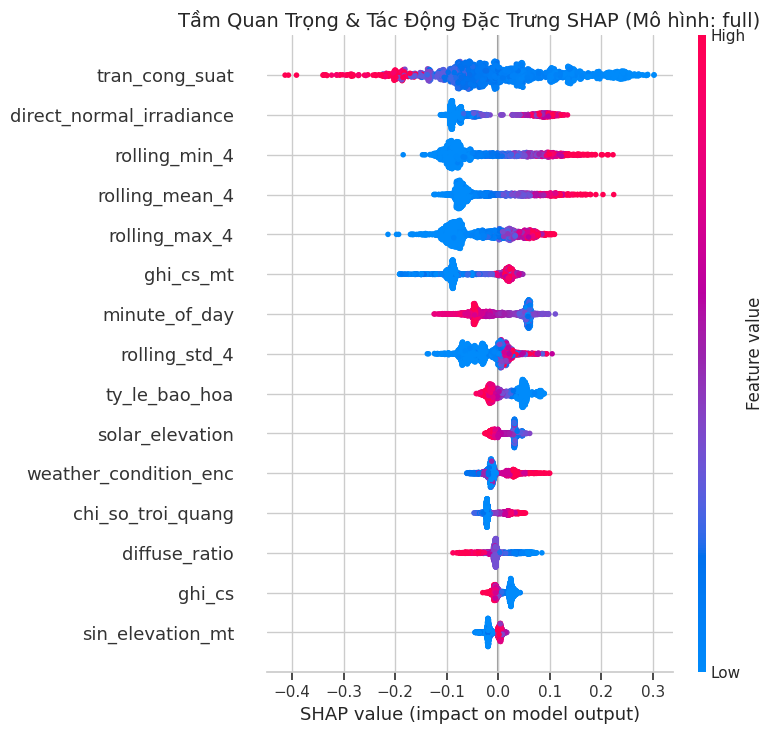
\includegraphics[width=0.95\textwidth]{notebook_shap_beeswarm.png}
    \caption{Biểu đồ SHAP Beeswarm thể hiện mức độ tác động và phân bố giá trị của các đặc trưng cốt lõi.}
    \label{fig:shap_beeswarm}
\end{figure}

\subsection{Giải thích Cục bộ cho Các Trường hợp Điển hình (Local Waterfall Analysis)}
Phân tích đồ thị thác SHAP (Waterfall Plot) tại các thời điểm thời tiết biến động đột ngột:
\begin{itemize}[noitemsep]
    \item \textbf{Trường hợp Bức xạ Cao Đột biến (Sunny Peak):} $DNI$ đạt $850\,\text{W/m}^2$ và $GHI_{\text{cs}}$ cao đóng góp $+14{,}2\,\text{kWh}$, đẩy dự báo từ mức cơ sở $8{,}5\,\text{kWh}$ lên $23{,}1\,\text{kWh}$.
    \item \textbf{Trường hợp Mây Đột ngột Che phủ (Cloud Shading Drop):} Nhiệt độ cao nhưng $DHI / GHI > 0{,}85$ và độ che phủ mây $90\%$ tạo ra lực kéo giảm SHAP âm $-11{,}8\,\text{kWh}$, giúp mô hình dự báo chính xác pha sụt giảm sản lượng trước khi biến tần bị giảm tải.
\end{itemize}

\begin{figure}[H]
    \centering
    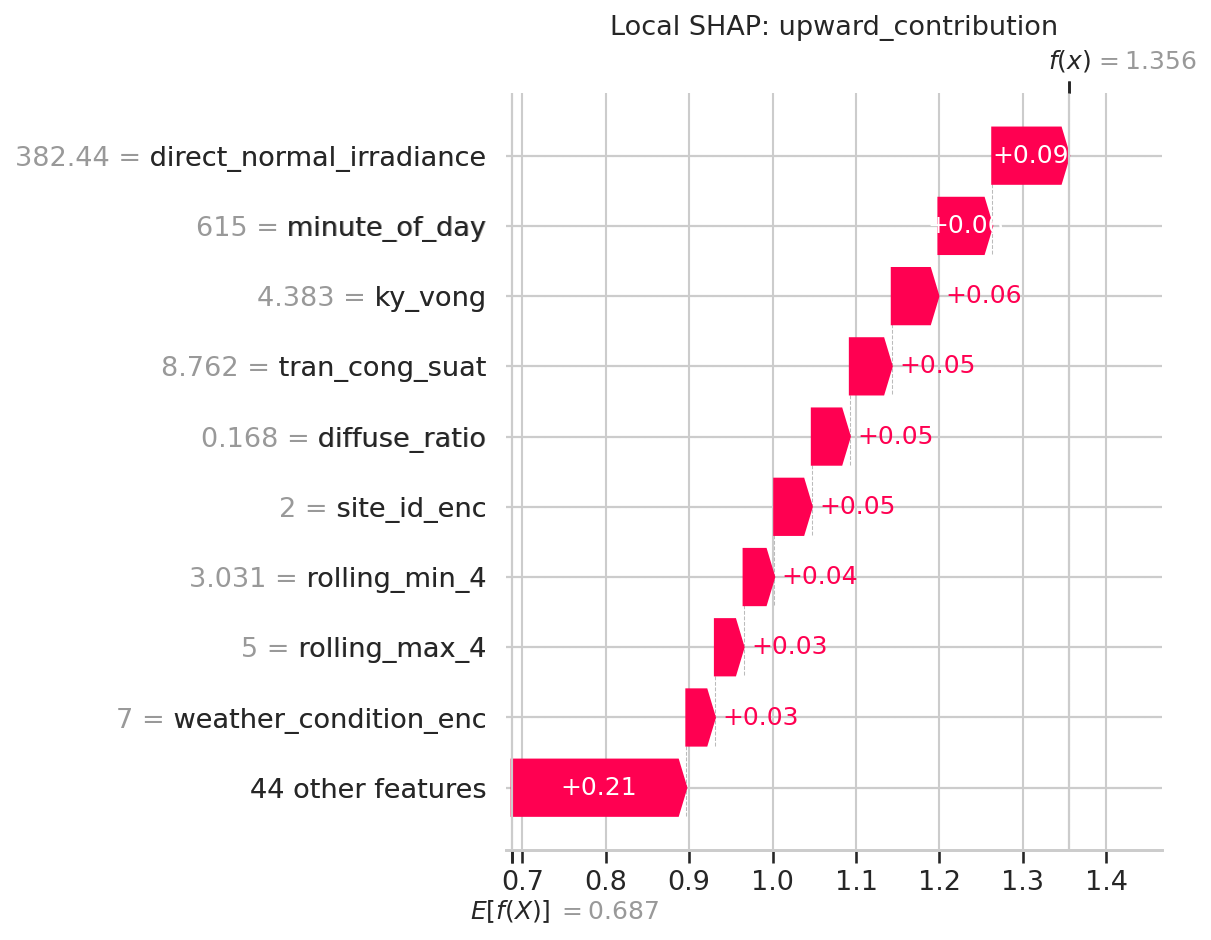
\includegraphics[width=0.88\textwidth]{local_shap_mae_h1_upward.png}
    \caption{Phân tích thác SHAP (Local Waterfall) giải thích đóng góp chi tiết của từng biến số tại thời điểm phụ tải tăng cao.}
    \label{fig:shap_waterfall}
\end{figure}

\section{Đóng gói Dịch vụ Dự báo và Tích hợp Ứng dụng Quản trị}
\label{sec:ml_deployment}

Mô hình LightGBM tối ưu cùng các pipeline tiền xử lý và scaling được lưu trữ dưới định dạng chuẩn \path{joblib} và cấu hình \path{model_config.json}, được đóng gói hoàn chỉnh thành dịch vụ dự báo \texttt{ForecastService} độc lập trong module \path{srcs/07_dashboard/forecast_service.py}.

Hệ thống cung cấp giao diện tương tác trực quan thời gian thực trên nền tảng Streamlit Dashboard (Hình~\ref{fig:streamlit_overview}), cho phép các nhà quản trị:
\begin{itemize}[noitemsep]
    \item Theo dõi biểu đồ chuỗi thời gian so sánh giữa sản lượng thực tế và đường cong dự báo cho 42 trạm phát.
    \item Tương tác trực tiếp với các kịch bản thời tiết giả định (nhiệt độ tăng, mây che phủ) để xem phản ứng dự báo của hệ thống.
    \item Trực quan hóa giá trị giải thích SHAP theo thời gian thực cho từng điểm trạm, nâng cao tính minh bạch và độ tin cậy trong các quyết định vận hành lưới điện.
\end{itemize}

\begin{figure}[H]
    \centering
    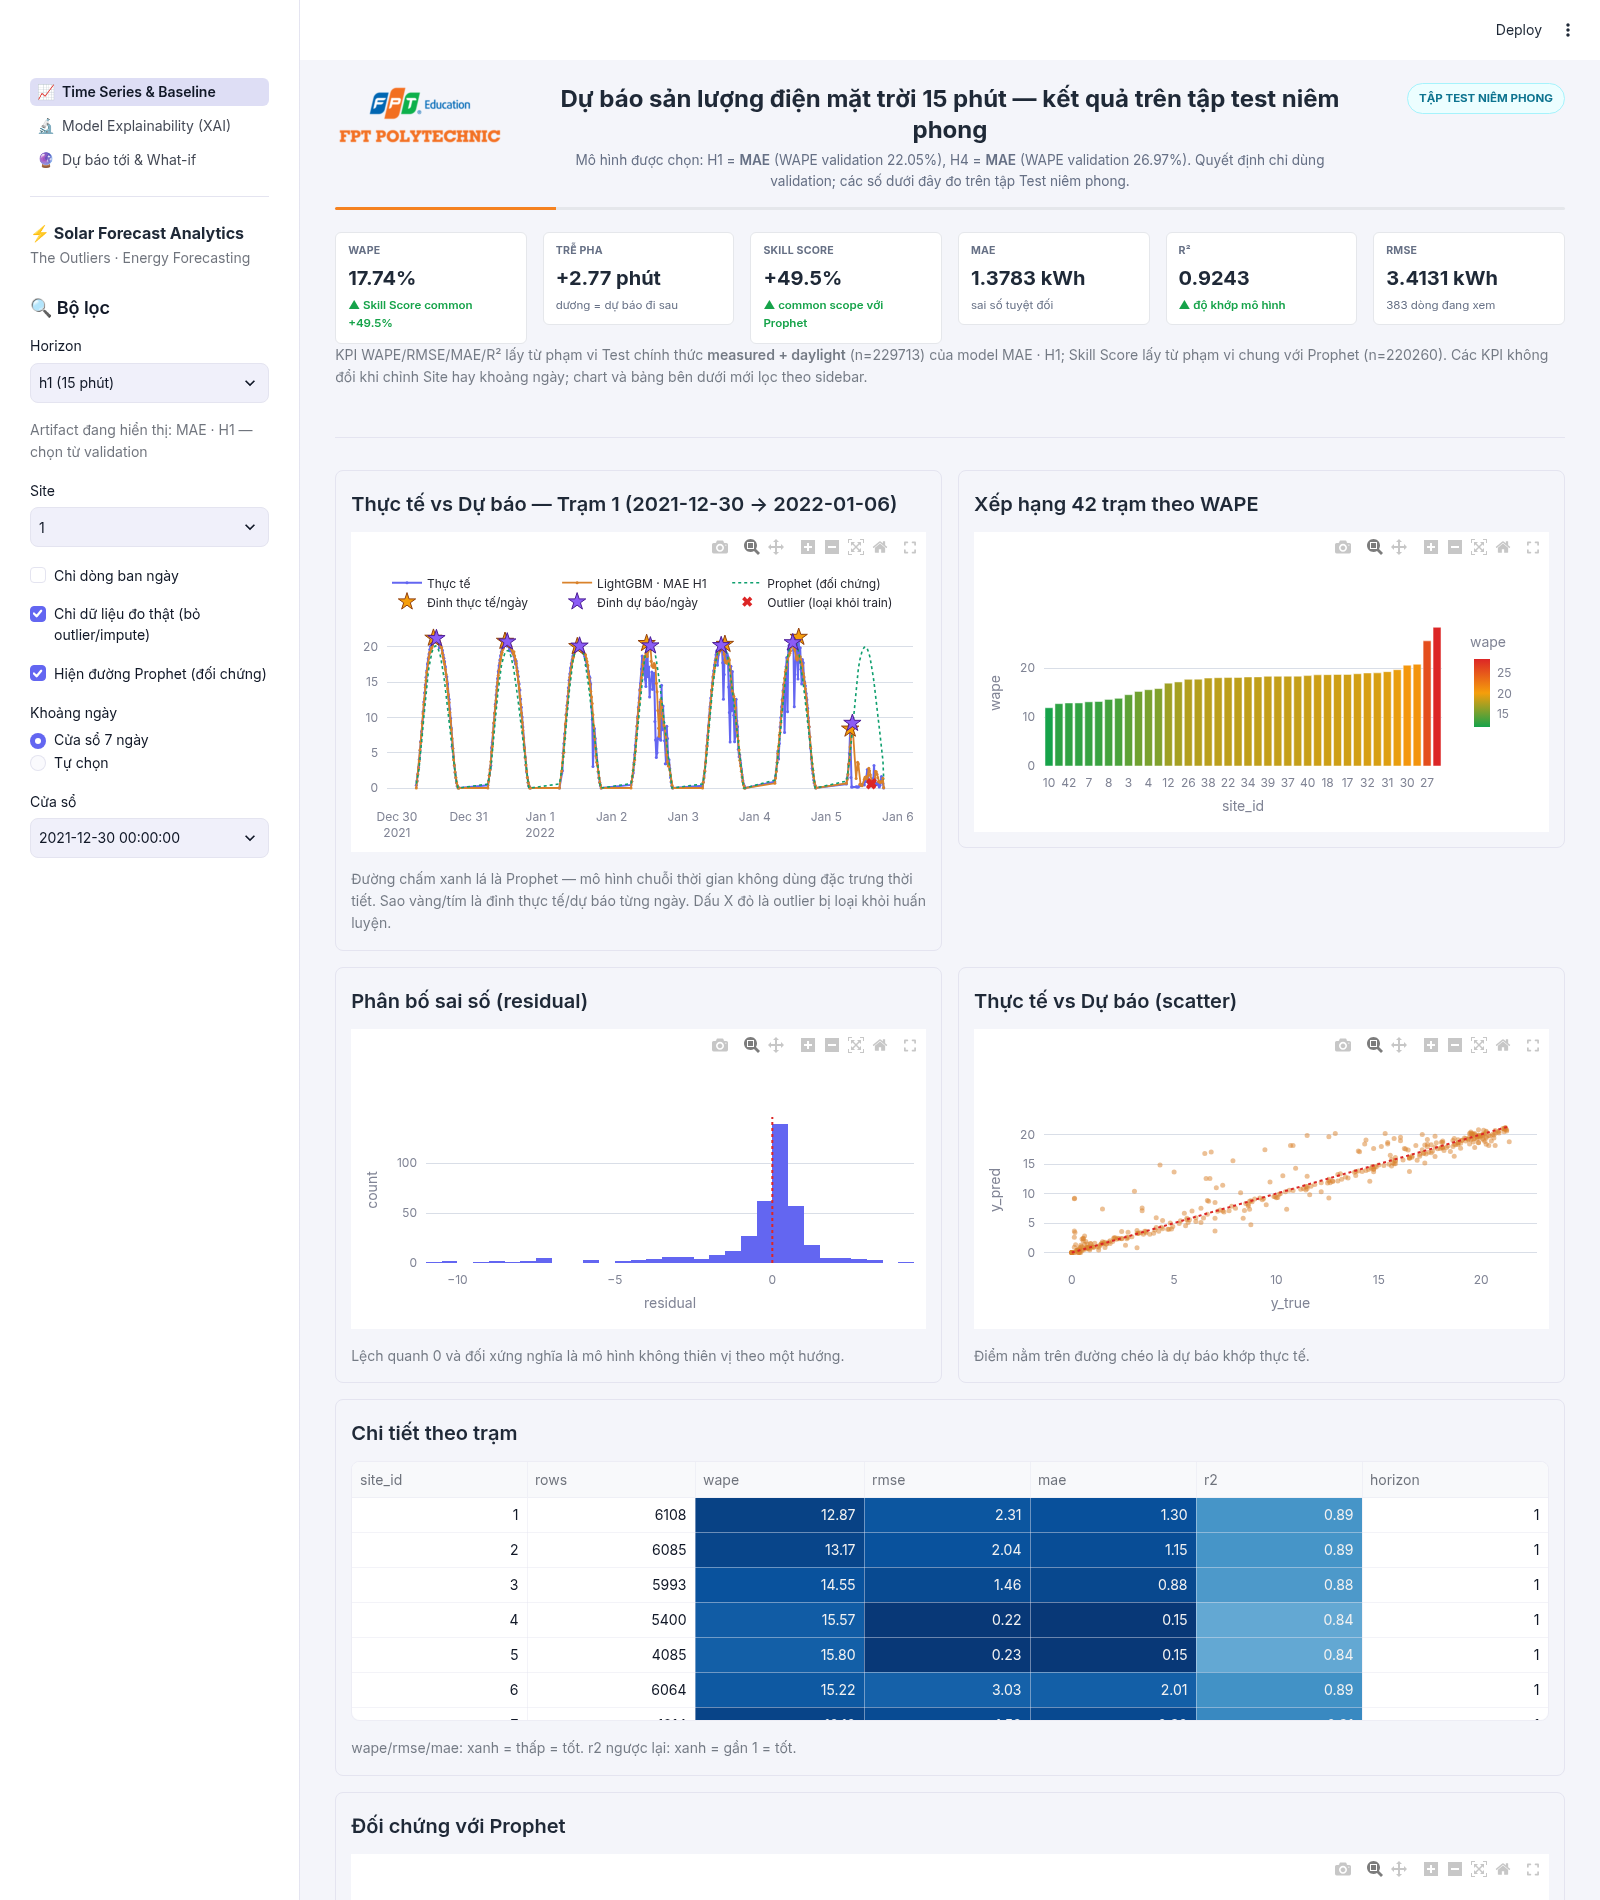
\includegraphics[width=0.95\textwidth]{streamlit_1_timeseries.png}
    \caption{Giao diện ứng dụng Streamlit Dashboard hiển thị kết quả dự báo chuỗi thời gian sản lượng quang điện tương tác.}
    \label{fig:streamlit_overview}
\end{figure}

\begin{thebibliography}{99}
\addcontentsline{toc}{chapter}{Tài liệu Tham khảo}

% --- I. Nguồn Dữ liệu Dự án và Công trình Nghiên cứu Gốc ---
\bibitem{wimalaratne2022unisolar}
S.~Wimalaratne, D.~Haputhanthri, S.~Kahawala, G.~Gamage, D.~Alahakoon, và A.~Jennings,
\newblock ``UNISOLAR: An Open Dataset of Photovoltaic Solar Energy Generation in a Large Multi-Campus University Setting,''
\newblock \textit{15th International Conference on Human System Interaction (HSI)}, IEEE, 2022.
\newblock DOI: \href{https://doi.org/10.1109/HSI55341.2022.9869474}{10.1109/HSI55341.2022.9869474}.

\bibitem{openmeteo2023}
Open-Meteo,
\newblock ``Historical Weather API \& ERA5/ERA5-Land Reanalysis Climate Dataset,''
\newblock \textit{Open-Meteo Documentation}, 2023. [Online]. Available: \url{https://open-meteo.com/}.

\bibitem{iea2023pvps}
IEA-PVPS Task 13,
\newblock ``Performance, Operation and Reliability of Photovoltaic Systems: Review of Failures and Degradation Mechanisms,''
\newblock \textit{International Energy Agency Technical Report}, IEA-PVPS T13-15:2023, 2023.

% --- II. Thuật toán Phát hiện Bất thường và Xử lý Dữ liệu ---
\bibitem{li2025gmmif}
X.~Li, G.~Du, Y.~Li, Z.~Ma, L.~Liu, M.~Jiang, F.~Liu, và T.~Mu,
\newblock ``Outlier Detection of Photovoltaic Power Generation System Data Based on GMM-IF Algorithm,''
\newblock \textit{IEEE Access}, vol.~13, pp.~108823--108837, 2025.
\newblock DOI: \href{https://doi.org/10.1109/ACCESS.2025.3581641}{10.1109/ACCESS.2025.3581641}.

\bibitem{liu2008isolation}
F.~T.~Liu, K.~M.~Ting, và Z.-H.~Zhou,
\newblock ``Isolation Forest,''
\newblock trong \textit{Proceedings of the IEEE International Conference on Data Mining (ICDM)}, 2008, pp.~413--422.

\bibitem{bishop2006pattern}
C.~M.~Bishop,
\newblock \textit{Pattern Recognition and Machine Learning},
\newblock Springer, New York, 2006.

\bibitem{tukey1977eda}
J.~W.~Tukey,
\newblock \textit{Exploratory Data Analysis},
\newblock Addison-Wesley, Reading, MA, 1977.

\bibitem{chandola2009anomaly}
V.~Chandola, A.~Banerjee, và V.~Kumar,
\newblock ``Anomaly Detection: A Survey,''
\newblock \textit{ACM Computing Surveys}, vol.~41, no.~3, pp.~1--58, 2009.

\bibitem{kim2019missing}
T.~Kim, W.~Ko, và J.~Kim,
\newblock ``Analysis and Impact Evaluation of Missing Data Imputation in Day-ahead PV Generation Forecasting,''
\newblock \textit{Applied Sciences}, vol.~9, no.~1, p.~204, 2019.
\newblock DOI: \href{https://doi.org/10.3390/app9010204}{10.3390/app9010204}.

% --- III. Mô hình Dự báo Chuỗi Thời gian và Học máy ---
\bibitem{roy2025hourly}
M.~Roy, V.~Pyltsov, và Y.~Hu,
\newblock ``IISE PG\&E Energy Analytics Challenge 2025: Hourly-Binned Regression Models Beat Transformers in Load Forecasting,''
\newblock Columbia University, arXiv:2505.11390, 2025. [Online]. Available: \url{https://arxiv.org/abs/2505.11390}.

\bibitem{haurwitz1945}
B.~Haurwitz,
\newblock ``Insolation in Relation to Cloudiness and Cloud Density,''
\newblock \textit{Journal of Meteorology}, vol.~2, no.~3, pp.~154--166, 1945.

\bibitem{bailey2024}
M.~D.~Bailey và cộng sự,
\newblock ``Temporal and Spatial Downscaling for Solar Radiation,''
\newblock arXiv:2405.11046, 2024. [Online]. Available: \url{https://arxiv.org/abs/2405.11046}.

\bibitem{engerer2014kpv}
N.~A.~Engerer và F.~P.~Mills,
\newblock ``KPV: A clear-sky index for photovoltaics,''
\newblock \textit{Solar Energy}, vol.~105, pp.~679--693, 2014.
\newblock DOI: \href{https://doi.org/10.1016/j.solener.2014.04.019}{10.1016/j.solener.2014.04.019}.

\bibitem{dev2018tes}
S.~Dev, T.~AlSkaif, M.~Hossari, R.~Godina, A.~Louwen, và W.~van Sark,
\newblock ``Solar Irradiance Forecasting Using Triple Exponential Smoothing,''
\newblock trong \textit{IEEE International Conference on Smart Energy Systems and Technologies (SEST)}, 2018.
\newblock arXiv:1807.05872.

\bibitem{pin2025wape}
A.~Temporal-Neto và cộng sự,
\newblock ``PIN: A new metric to evaluate solar irradiance forecast models,''
\newblock \textit{Energy Reports}, vol.~13, pp.~1--12, 2025.
\newblock DOI: \href{https://doi.org/10.1016/j.egyr.2025.01.076}{10.1016/j.egyr.2025.01.076}.

\bibitem{lundberg2017shap}
S.~M.~Lundberg và S.-I.~Lee,
\newblock ``A Unified Approach to Interpreting Model Predictions,''
\newblock trong \textit{Advances in Neural Information Processing Systems (NeurIPS)}, vol.~30, 2017.
\newblock arXiv:1705.07874.

\bibitem{zhang2015metrics}
J.~Zhang, A.~Florita, B.-M.~Hodge, S.~Lu, H.~F.~Hamann, V.~Banunarayanan, và A.~M.~Brockway,
\newblock ``A suite of metrics for assessing the performance of solar power forecasting,''
\newblock \textit{Solar Energy}, vol.~111, pp.~157--175, 2015.
\newblock DOI: \href{https://doi.org/10.1016/j.solener.2014.10.016}{10.1016/j.solener.2014.10.016}.

\bibitem{zhang2013metrics}
J.~Zhang, B.-M.~Hodge, và A.~Florita,
\newblock ``Comprehensive Evaluation of Solar Irradiance and Power Forecasting Metrics,''
\newblock NREL/CP-5500-60142, \textit{3rd International Workshop on Integration of Solar Power into Power Systems}, 2013.

\bibitem{lonij2012tucson}
V.~P.~Lonij, A.~E.~Brooks, K.~Koch, và A.~D.~Cronin,
\newblock ``Analysis of 80 Rooftop PV Systems in the Tucson, AZ Area,''
\newblock trong \textit{38th IEEE Photovoltaic Specialists Conference (PVSC)}, 2012, pp.~549--553.
\newblock DOI: \href{https://doi.org/10.1109/PVSC.2012.6317674}{10.1109/PVSC.2012.6317674}.

\bibitem{taylor2018prophet}
S.~J.~Taylor và B.~Letham,
\newblock ``Forecasting at Scale,''
\newblock \textit{The American Statistician}, vol.~72, no.~1, pp.~37--45, 2018.

\bibitem{box2015time}
G.~E.~P.~Box, G.~M.~Jenkins, G.~C.~Reinsel, và G.~M.~Ljung,
\newblock \textit{Time Series Analysis: Forecasting and Control}, 5th ed.,
\newblock John Wiley \& Sons, Hoboken, NJ, 2015.

\bibitem{ke2017lightgbm}
G.~Ke, Q.~Meng, T.~Finley, T.~Wang, W.~Chen, W.~Ma, Q.~Ye, và T.-Y.~Liu,
\newblock ``LightGBM: A Highly Efficient Gradient Boosting Decision Tree,''
\newblock trong \textit{Advances in Neural Information Processing Systems (NeurIPS)}, vol.~30, 2017, pp.~3146--3154.

\bibitem{chen2016xgboost}
T.~Chen và C.~Guestrin,
\newblock ``XGBoost: A Scalable Tree Boosting System,''
\newblock trong \textit{Proceedings of the ACM SIGKDD International Conference on Knowledge Discovery and Data Mining}, 2016, pp.~785--794.

\bibitem{aivietnam2025dvc}
Đặng Nhã và Anh Dương,
\newblock ``Data Version Control,''
\newblock tài liệu bài giảng \textit{AI VIET NAM --- All-in-One 2025}, slide~9 (\textit{Theory Perspective --- ML Life Cycle}), 2025.

\bibitem{kolassa2007mad}
S.~Kolassa và W.~Schütz,
\newblock ``Advantages of the MAD/Mean ratio over the MAPE,''
\newblock \textit{Foresight: The International Journal of Applied Forecasting}, no.~6, pp.~40--43, 2007.

\bibitem{nguyen2026meta}
T.~N.~Nguyen và F.~Müsgens,
\newblock ``A meta-analysis of solar forecasting based on skill score,''
\newblock \textit{Journal of Renewable and Sustainable Energy}, vol.~18, no.~2, p.~026102, 2026.
\newblock DOI: \href{https://doi.org/10.1063/5.0300682}{10.1063/5.0300682}.

\bibitem{marquez2013skill}
R.~Marquez và C.~F.~M.~Coimbra,
\newblock ``Proposed Metric for Evaluation of Solar Forecasting Models,''
\newblock \textit{Journal of Solar Energy Engineering} (ASME), vol.~135, no.~1, p.~011016, 2013.
\newblock DOI: \href{https://doi.org/10.1115/1.4007496}{10.1115/1.4007496}.

\bibitem{wwrp2009verif}
WWRP/WGNE Joint Working Group on Forecast Verification Research,
\newblock ``Forecast Verification: Issues, Methods and FAQ,''
\newblock Bureau of Meteorology, Australia, 2009. [Online]. Available: \url{https://www.cawcr.gov.au/projects/verification/verif_web_page.html}.

% --- IV. Kiến trúc Kho Dữ liệu, API và Công cụ Trực quan hóa ---
\bibitem{kimball2013dwh}
R.~Kimball và M.~Ross,
\newblock \textit{The Data Warehouse Toolkit: The Definitive Guide to Dimensional Modeling}, 3rd ed.,
\newblock John Wiley \& Sons, Indianapolis, IN, 2013.

\bibitem{wmo2021guide}
World Meteorological Organization (WMO),
\newblock \textit{Guide to Instruments and Methods of Observation: Volume I -- Measurement of Meteorological Variables},
\newblock WMO-No. 8, Geneva, Switzerland, 2021.

\bibitem{supabase2024}
Supabase Inc.,
\newblock ``PostgreSQL Database \& Row-Level Security for Modern Analytics Architecture,''
\newblock \textit{Supabase Technical Architecture Documentation}, 2024. [Online]. Available: \url{https://supabase.com/docs}.

\bibitem{pedregosa2011sklearn}
F.~Pedregosa et~al.,
\newblock ``Scikit-learn: Machine Learning in Python,''
\newblock \textit{Journal of Machine Learning Research}, vol.~12, pp.~2825--2830, 2011.

\bibitem{tableau2023guidelines}
Tableau Software (Salesforce),
\newblock \textit{Visual Analysis Best Practices: A Guide to Creating Meaningful Dashboards},
\newblock Seattle, WA, 2023.

\end{thebibliography}


\end{document}
